\documentclass[border=10pt]{standalone}
\usepackage{tikz}
\usetikzlibrary{shapes.geometric, arrows.meta, positioning, fit, backgrounds, calc}

\definecolor{rustcolor}{HTML}{DEA584}
\definecolor{corecolor}{HTML}{4A90D9}
\definecolor{storecolor}{HTML}{50C878}
\definecolor{netcolor}{HTML}{9B59B6}
\definecolor{clicolor}{HTML}{E74C3C}
\definecolor{cryptocolor}{HTML}{F39C12}
\definecolor{serdecolor}{HTML}{1ABC9C}
\definecolor{asynccolor}{HTML}{E91E63}
\definecolor{testcolor}{HTML}{607D8B}
\definecolor{bglight}{HTML}{F8F9FA}

\begin{document}
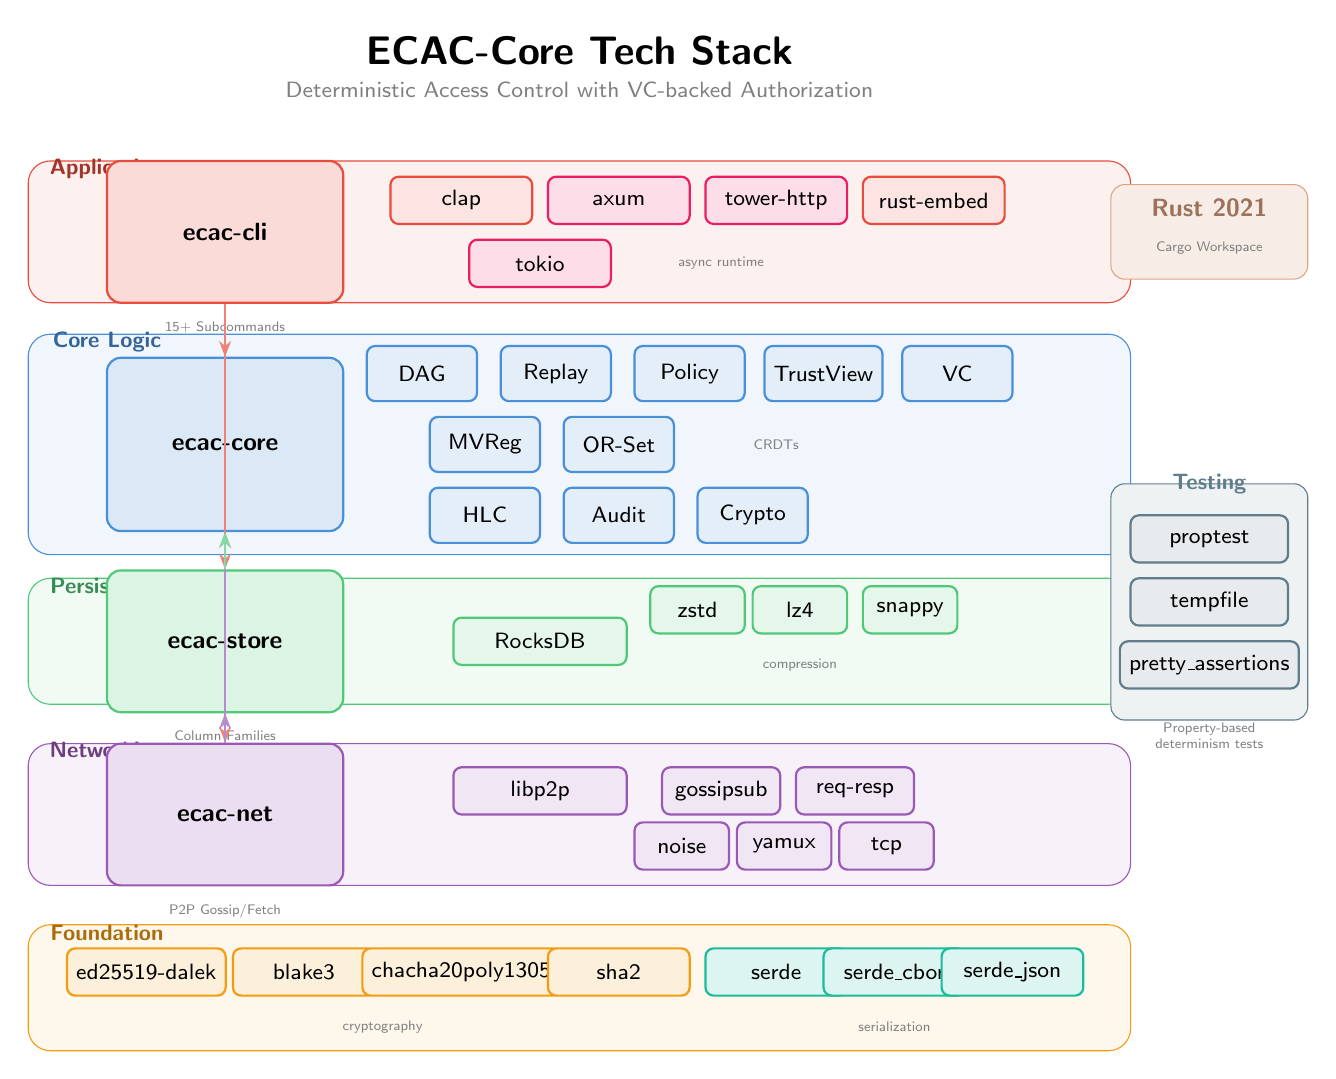
\begin{tikzpicture}[
    node distance=0.8cm and 1.2cm,
    box/.style={rectangle, rounded corners=3pt, draw=#1, fill=#1!15,
                minimum width=2.2cm, minimum height=0.7cm,
                font=\footnotesize\sffamily, align=center, thick},
    crate/.style={rectangle, rounded corners=5pt, draw=#1, fill=#1!20,
                  minimum width=3cm, minimum height=1.8cm,
                  font=\small\sffamily\bfseries, thick},
    layer/.style={rectangle, rounded corners=8pt, draw=#1, fill=#1!8,
                  minimum width=14cm, font=\sffamily\bfseries},
    dep/.style={box=#1, minimum width=1.8cm, minimum height=0.6cm},
    arrow/.style={-{Stealth[length=2mm]}, thick, #1}
]

% Title
\node[font=\Large\sffamily\bfseries] (title) at (0, 5.5) {ECAC-Core Tech Stack};
\node[font=\footnotesize\sffamily, text=gray] at (0, 5.0) {Deterministic Access Control with VC-backed Authorization};

% === Application Layer ===
\node[layer=clicolor, minimum height=1.8cm] (applayer) at (0, 3.2) {};
\node[font=\footnotesize\sffamily\bfseries, text=clicolor!70!black] at (-6, 4.0) {Application};

\node[crate=clicolor] (cli) at (-4.5, 3.2) {\textbf{ecac-cli}};
\node[font=\tiny\sffamily, text=gray, below=0.1cm of cli.south] {15+ Subcommands};

\node[dep=clicolor] (clap) at (-1.5, 3.6) {clap};
\node[dep=asynccolor] (axum) at (0.5, 3.6) {axum};
\node[dep=asynccolor] (towerhttp) at (2.5, 3.6) {tower-http};
\node[dep=clicolor] (rustembed) at (4.5, 3.6) {rust-embed};

\node[dep=asynccolor] (tokio) at (-0.5, 2.8) {tokio};
\node[font=\tiny\sffamily, text=gray] at (1.8, 2.8) {async runtime};

% === Core Layer ===
\node[layer=corecolor, minimum height=2.8cm] (corelayer) at (0, 0.5) {};
\node[font=\footnotesize\sffamily\bfseries, text=corecolor!70!black] at (-6, 1.8) {Core Logic};

\node[crate=corecolor, minimum height=2.2cm] (core) at (-4.5, 0.5) {\textbf{ecac-core}};

% Core modules
\node[box=corecolor, minimum width=1.4cm] (dag) at (-2, 1.4) {DAG};
\node[box=corecolor, minimum width=1.4cm] (replay) at (-0.3, 1.4) {Replay};
\node[box=corecolor, minimum width=1.4cm] (policy) at (1.4, 1.4) {Policy};
\node[box=corecolor, minimum width=1.4cm] (trustview) at (3.1, 1.4) {TrustView};
\node[box=corecolor, minimum width=1.4cm] (vc) at (4.8, 1.4) {VC};

\node[box=corecolor, minimum width=1.4cm] (mvreg) at (-1.2, 0.5) {MVReg};
\node[box=corecolor, minimum width=1.4cm] (orset) at (0.5, 0.5) {OR-Set};
\node[font=\tiny\sffamily, text=gray] at (2.5, 0.5) {CRDTs};

\node[box=corecolor, minimum width=1.4cm] (hlc) at (-1.2, -0.4) {HLC};
\node[box=corecolor, minimum width=1.4cm] (audit) at (0.5, -0.4) {Audit};
\node[box=corecolor, minimum width=1.4cm] (crypto) at (2.2, -0.4) {Crypto};

% === Persistence Layer ===
\node[layer=storecolor, minimum height=1.6cm] (storelayer) at (0, -2.0) {};
\node[font=\footnotesize\sffamily\bfseries, text=storecolor!70!black] at (-6, -1.3) {Persistence};

\node[crate=storecolor] (store) at (-4.5, -2.0) {\textbf{ecac-store}};
\node[font=\tiny\sffamily, text=gray, below=0.1cm of store.south] {Column Families};

\node[dep=storecolor, minimum width=2.2cm] (rocksdb) at (-0.5, -2.0) {RocksDB};
\node[dep=storecolor, minimum width=1.2cm] (zstd) at (1.5, -1.6) {zstd};
\node[dep=storecolor, minimum width=1.2cm] (lz4) at (2.8, -1.6) {lz4};
\node[dep=storecolor, minimum width=1.2cm] (snappy) at (4.2, -1.6) {snappy};
\node[font=\tiny\sffamily, text=gray] at (2.8, -2.3) {compression};

% === Network Layer ===
\node[layer=netcolor, minimum height=1.8cm] (netlayer) at (0, -4.2) {};
\node[font=\footnotesize\sffamily\bfseries, text=netcolor!70!black] at (-6, -3.4) {Networking};

\node[crate=netcolor] (net) at (-4.5, -4.2) {\textbf{ecac-net}};
\node[font=\tiny\sffamily, text=gray, below=0.1cm of net.south] {P2P Gossip/Fetch};

\node[dep=netcolor, minimum width=2.2cm] (libp2p) at (-0.5, -3.9) {libp2p};
\node[dep=netcolor, minimum width=1.5cm] (gossipsub) at (1.8, -3.9) {gossipsub};
\node[dep=netcolor, minimum width=1.5cm] (reqresp) at (3.5, -3.9) {req-resp};
\node[dep=netcolor, minimum width=1.2cm] (noise) at (1.3, -4.6) {noise};
\node[dep=netcolor, minimum width=1.2cm] (yamux) at (2.6, -4.6) {yamux};
\node[dep=netcolor, minimum width=1.2cm] (tcp) at (3.9, -4.6) {tcp};

% === Foundation (Crypto & Serialization) ===
\node[layer=cryptocolor, minimum height=1.6cm] (foundlayer) at (0, -6.4) {};
\node[font=\footnotesize\sffamily\bfseries, text=cryptocolor!70!black] at (-6, -5.7) {Foundation};

\node[dep=cryptocolor] (ed25519) at (-5.5, -6.2) {ed25519-dalek};
\node[dep=cryptocolor] (blake3) at (-3.5, -6.2) {blake3};
\node[dep=cryptocolor] (chacha) at (-1.5, -6.2) {chacha20poly1305};
\node[dep=cryptocolor] (sha2) at (0.5, -6.2) {sha2};
\node[font=\tiny\sffamily, text=gray] at (-2.5, -6.9) {cryptography};

\node[dep=serdecolor] (serde) at (2.5, -6.2) {serde};
\node[dep=serdecolor] (cbor) at (4.0, -6.2) {serde\_cbor};
\node[dep=serdecolor] (json) at (5.5, -6.2) {serde\_json};
\node[font=\tiny\sffamily, text=gray] at (4.0, -6.9) {serialization};

% === Testing sidebar ===
\node[rectangle, rounded corners=5pt, draw=testcolor, fill=testcolor!10,
      minimum width=2.5cm, minimum height=3cm] (testing) at (8, -1.5) {};
\node[font=\footnotesize\sffamily\bfseries, text=testcolor] at (8, 0) {Testing};
\node[dep=testcolor, minimum width=2cm] (proptest) at (8, -0.7) {proptest};
\node[dep=testcolor, minimum width=2cm] (tempfile) at (8, -1.5) {tempfile};
\node[dep=testcolor, minimum width=2cm] (prettyassert) at (8, -2.3) {pretty\_assertions};
\node[font=\tiny\sffamily, text=gray, text width=2cm, align=center] at (8, -3.2) {Property-based\\determinism tests};

% === Rust/Cargo badge ===
\node[rectangle, rounded corners=5pt, draw=rustcolor, fill=rustcolor!20,
      minimum width=2.5cm, minimum height=1.2cm] (rust) at (8, 3.2) {};
\node[font=\small\sffamily\bfseries, text=rustcolor!70!black] at (8, 3.5) {Rust 2021};
\node[font=\tiny\sffamily, text=gray] at (8, 3.0) {Cargo Workspace};

% === Arrows (dependencies) ===
\draw[arrow=clicolor!70] (cli.south) -- ++(0,-0.3) -| (core.north);
\draw[arrow=clicolor!70] (cli.south) -- ++(0,-0.5) -| (store.north);
\draw[arrow=clicolor!70] (cli.south) -- ++(0,-0.7) -| (net.north);

\draw[arrow=netcolor!70] (net.north) -- ++(0,0.5) -| (core.south);
\draw[arrow=netcolor!70] (net.north) -- ++(0,0.3) -| (store.south);

\draw[arrow=storecolor!70] (store.north) -- ++(0,0.3) -| (core.south);

\end{tikzpicture}
\end{document}
